\documentclass{beamer}
\usetheme{default}
\begin{document}

\begin{frame}{Atomic Orbitals}

Atomic wavefunctions can be written as:
\[
    \psi_{nlm}({\bf x}) = R_{nl}(r) Y_{lm}(\Omega)
\]
we plot $| \psi_{nlm}({\bf x})|^2$ for Radium (Z=88) with electronic
configuration: $1s^2 2s^2 2p^6 3s^2 3p^6 3d^{10} 4s^2 4p^6 5s^2 4d^{10}
5p^6 4f^{14} 5d^{10} 6s^2 6p^6 7s^2$

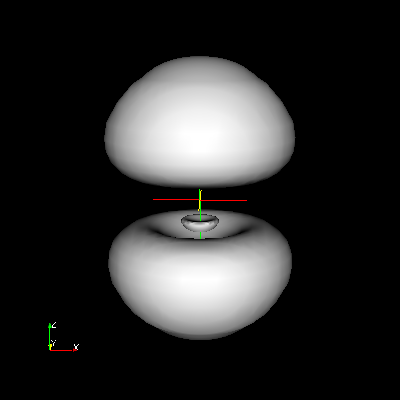
\includegraphics[width=1in]{../img/orbital_n6l1m0.png}
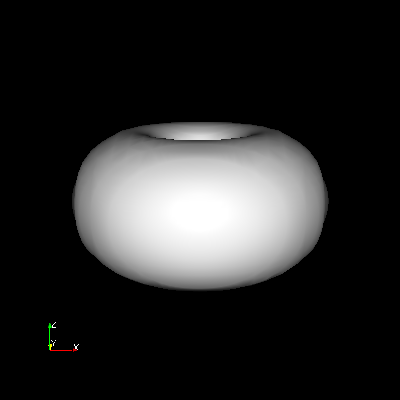
\includegraphics[width=1in]{../img/orbital_n5l2m2.png}
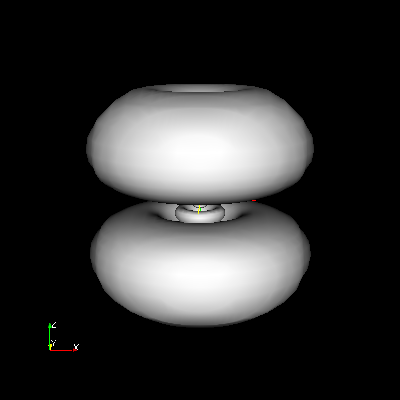
\includegraphics[width=1in]{../img/orbital_n5l2m1.png}
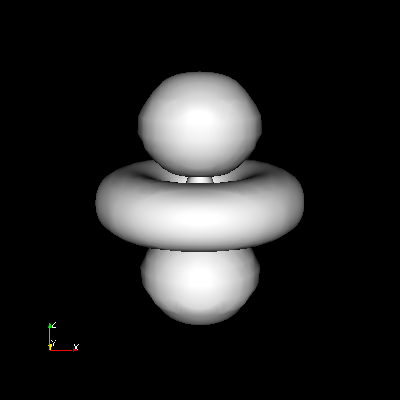
\includegraphics[width=1in]{../img/orbital_n5l2m0.png}

From left to right $(n l m)$: 610, 522, 521, 520

\end{frame}

\begin{frame}{More Details}

We are solving the atomic Hartree-Fock equations:
\[
    HF
\]

\end{frame}

\end{document}
